Convolutional Neural network's (CNN) main goal is to make a computer recognize images and objects. For such, it is primarily used for image classification or object recognition.

CNN was inspired by the biological processes of the human brain. Its connectivity patterns resemble the human's visual cortex. But an image is perceived differently by a human brain than by a computer. To a computer, an image is interpreted as an array of numbers. Thus CNN is designed to work with two-dimensional image arrays, although it is possible to work with one-dimensional or three-dimensional arrays too \cite{mlmastery}.

CNN is a variation of FNN \cite{Goodfellow-et-al-2016}. It usually consists of the input layer followed by multiple hidden layers, typically several \textit{convolutional layers} with standard \textit{pooling layers}, and ending with the output layer. 

\setsecnumdepth{all}
\subsubsection{Convolutional Layer}

The convolutional layer's objective is to extract key features from the input image by passing a matrix known as a \textit{kernel} over the input image abstracted into a matrix \cite{mathworkscnn}.

\begin{figure}[h]
	\centering
    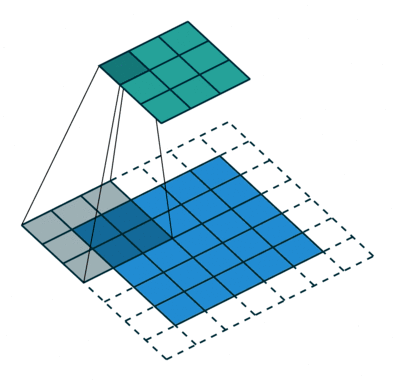
\includegraphics[width=8cm]{conv_layer_padding.png}
	\caption{Convolution of an 5x5x1 image with 3x3x1 kernel \cite{compguideCnn}}
	\label{fig:cnn_conv}
\end{figure}


The convolution result can be of two types depending on their size. One being the convoluted feature is reduced in dimensions compared to the input, which is called \textit{valid padding}. For example, an input image of dimensions 8x8 being reduced to 6x6 after convolution operation, and the other type being where dimensions are either increased or remain the same, which is called \textit{same padding} \cite{compguideCnn}.

\subsubsection{Pooling Layer}


Similar to the previously mentioned convolutional layer, the pooling layer reduces the convolved feature's spatial size to decrease the computational power required for data processing. Furthermore, being useful by extracting dominant features, which are rotational and positional invariant, thus maintaining the process of effectively training the model \cite{compguideCnn}.

There are two types of pooling: \textit{max pooling} and \textit{average pooling}. Max pooling returns the maximum value from the portion of the image covered by the kernel. It performs as a noise suppressant, discarding the noisy activations altogether and performing de-noising and dimensionality reduction. Where average pooling returns the average of all the values from the same covered portion, performing dimensionality reduction as a noise suppressing mechanism. Hence, it is possible to note that max-pooling performs better \cite{compguideCnn}.

\begin{figure}[h]
	\centering
    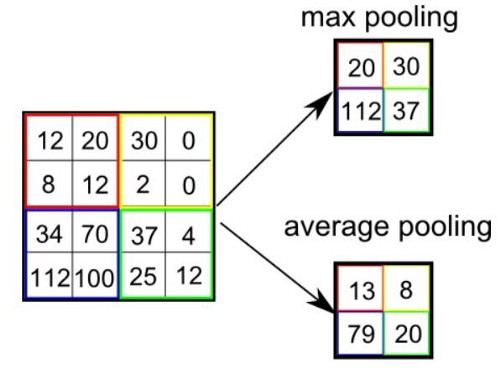
\includegraphics[width=8cm]{conv_pooling.png}
	\caption{Types of pooling \cite{compguideCnn}}
	\label{fig:cnn_pooling}
\end{figure}
